\section{Constructing the Network}\label{sec:data}

\textbf{TODO} clean, sections 4.1 is now very redundant with previous sections.
Important section here is 4.4 (Trevor stuff!)

\subsection{Data sources and cleaning}

{\color{red} this section 2.1 should include a description of the 6 datasets we used---2 complaints, 2 shootings, roster, and unit reference---and how they were constructed. I did my best to pull the important info from the chicago manuscript here but I probably did a bad job }

{\color{red} right now this is a hodge podge of info I could find about how we dealt with the original data.}

The original dataset used in this study was a collection of
107,276 {\color{red} civilian?} complaints against officers of the CPD
from the years {\color{red} xx to xx}, and cover a range of types of
allegations, including First Amendment violations, wrongful arrest, illegal
search and seizure, excessive force, and more.
The dataset---which is now publicly available at \url{https://invisible.institute/police-data}---was 
originally obtained  by the Citizens Police Data Project at the Invisible
Institute and the University of Chicago Law School’s Mandel Legal Aid Clinic
via a Freedom of Information Act request and subsequent litigation \cite{xx}.

To guard against endogeneity problems,
we excluded all complaints  {\color{red}(\_\%)} connected in any way to the discharge of a
firearm. {\color{red} did we?}

For the period under study, the Independent Police Review Authority (IPRA)
handled initial responsibility for processing and investigating civilian
complaints. Filing a complaint
required civilians to swear out an affidavit attesting to the truth of their
allegations. Filing also required affidavits to be signed in person, at a
limited number of locations. After a filing was complete, the complaint was
investigated by an independent authority or other agency. For those
investigations that were completed, allegations were either sustained,
un-sustained or the officer was exonerated. 
Less than 3\% of complaints were
sustained, and officers were almost never disciplined. 




We first cleaned the civilian complaints to fill in missing information from
{\color{red} other records??? how?? what records?}. A significant number of complaints were missing any officer
identities, race, gender, dates of appointments and other information, and
another group of complaints were missing affidavits from the complainants. Our
dataset included 19,843 complaints involving 9,737 unique officers that had
complete information. {\color{red} after cleaning? or did we just throw out data with missing entries}

We obtained personnel records on all Chicago police officers for the relevant
time period January of 2008 to November 2015 by filing a Freedom of Information
Act (FOIA) request with City of Chicago Department of Human Resources. The
bi-annual personnel data include each officer's name, position title (rank),
and original hire date. We use the officers first and last name and the
original date of appointment to link records with the other datasets. 
{\color{red} all these dates seem wrong too...}
 
 We linked information across datasets (the civilian complaint dataset and the
shootings dataset) by constructing a unique identifier for each and every
officer on the roster. In the event that officers shared names, we verified the
officer’s identity through badge numbers and/or date of appointment where
available on either the relevant complaints or the shootings data from IPRA.

Officers listed in the complaints were identified using personnel records on
all Chicago police officers that had been separately obtained by filing a
Freedom of Information Act (FOIA) request with the City of Chicago Department
of Human Resources. The bi-annual personnel data include each officer's name,
position title (rank), and original hire date. These records were available
from 2002 to 2014. We used the officers’ badge number and the original hire
date to link records with the complaint and shooting datasets, and to identify
unique officers. 

\subsection{Officer social network}


We constructed a social network of CPD police officers over which a possible
contagion effect could be mediated
using the {\color{red} two complaints datasets with 19,843 complaints between Jan 2008 and Nov 2015}. 
In particular, we constructed a single undirected network that 
 connects every pair of officers who were listed together on any
 civilian complaint during the period of study. This complaint network
contains 9,737 unique officer nodes and 47,037 edges. We did not
weight the edges of our complaint network to reflect the number of times that a
pair of officers are listed together on the same civilian complaint. The vast
majority (83\%) of edges would have a weight of 1, corresponding to officers who 
appeared together on a complaint only once. The average officer received 1.72 complaints. 
Approximately 15\% of officers connect to 10 or more edges in the network, while the top
1\% of officers connect to 26 edges on average. {\color{red} replace this with a degree distribution plot}

The network contains several smaller components, many isolated
officers, and one very large connected component. As is true for most social network analysis, we use this
largest connected component as the focus of our study, and discard the remainder. 
The largest connected component in the complaint network contains 7,825 (80\%) of the
nodes, 46,568 (99\%) of the edges, and 418 (93\%) of the 450 shooting officers in %of the 450
the original larger network. 
As detailed in the Appendix, the LCC also has a similar
clustering coefficient, an average path length, and its degree distribution
follows a power-law distribution as is true for the larger network. 
{\color{red} again need plots}

From this point onward, the ``complaint''/``social network''  refers to the largest connected component.

\paragraph{Rationale and limitations}
If two officers are listed on a complaint together, they respond
to calls together and---as evidence suggests---engage in misconduct
together. Being listed on a complaint together also suggests a pre-existing
relationship through which scripts of violence could be transmitted.
Previous research suggests that
co-offending represents strong and enduring relationships between individuals \cite{Xx}.
We therefore treated co-offending as evidence of an existing relationship
between the two individuals involved, rather than as a point-in-time estimate
or marker of when that relationship formed. Thus, the social network we build
is \emph{static} over time: an edge indicates that two individuals have co-offended together
at least once at some time during the study period.

We study civilian-facing complaints in particular based on the assumption that 
officers who interact during civilian encounters are
significantly more likely to spread civilian-related response behaviors---such as violence---through
those interactions. In our data, 60.3\% of complaints were filed by civilians,
while the remaining 39.7\% were generated from within the department. 
Over 55\% of civilian complaints in our dataset name two or more officers,
indicating that the majority of alleged police misconduct occurs in a group
setting.

These data were not without limitations.
Civilians are generally not reliable reporters of the events in question in a complaint allegation;
reports suffer from civilian biases against the police, faulty memory and other
common sources of mistake or misreporting. 
Further, a large portion of potential police misconduct goes unreported by
civilians, frequently owing to administrative requirements but also owing to a
range of factors associated with a strong distrust of authority, a lack of
faith in accountability, and a reluctance to risk retaliation.  
We make no claims about civilian
complaints other than that the officers that are listed as subjects of the
complaints interacted with each other and with civilians in the encounter at
the reported place on the reported date. 
But even so, the complaint
co-offender network cannot be said to accurately represent the social
connections among officers; we capture a subset---but not the full set---of 
social connections among officers.

Finally, the subset of officers in the complaint network are not necessarily
representative of the larger population of police officers. If officers in the
complaint network differ from those not in the network, our results might not
represent actual contagion for the department. However, representativeness does 
not pose a strong concern because the majority of officers (70-75\%) and shooting officers (93\%)  are present in our 
network {\color{red} true of the LCC?}. Thus, the analysis captures a significant
fraction of both shooting and non-shooting officers. 
 But we cannot determine whether this network
is representative of other police departments outside of Chicago. 

\subsection{Officer shooting history}

We endowed each officer node in the social network with a history of shooting behaviour
using detailed incident-level data {\color{red} two shooting datasets}
collected by IPRA on police-involved shootings occurring between 2008 and
November 2015. Chicago city regulations required IPRA to investigate ``all cases
in which a department member discharges his or her firearm, stun gun, or Taser
in a manner which potentially could strike an individual, even if no allegation
of misconduct is made.'' CPD General Orders required officers to notify IPRA
each time a CPD member discharged a firearm. Once notified, IPRA created an
electronic record of its investigation by assigning each incident a log number
in CPD and IPRA’s electronic case management system (CLEAR). 

City regulations required IPRA to issue quarterly reports on weapons-discharge
investigations. In its reports, IPRA included five categories of
weapons-discharge notifications: “hit shooting” of firearm, “non-hit shooting”
of firearm, shooting of firearm at an animal, shootings with taser, and
oleoresin capsicum (OC). We concentrate analysis on the first category of data
consisting of police-involved “hit shootings” (meaning shootings that hit a
civilian) with a firearm, from January 2008 to November 2015. 

Reports provided detailed incident-level information from these categories. Key
variables in this dataset included: the date and location of the shooting,
identifying information associated with the officers who had discharged their
gun, and information about the organizational assignment of the relevant
officer. Individual officers involved in police shootings were linked through a
unique identifying number to those officers in civilian complaints.

We excluded both same-day same-event shootings, involving connected officers
who were involved in a police shooting at the same event, and same-day
different event shootings. Excluding the latter (for now) biases our
investigation in a conservative direction against a finding; same-day different
event shootings are likely to reflect contagion, particularly in light of the
short period of time between shootings.

In the shootings network, nodes in the graph represent individual shootings,
meaning a discharge of a firearm by an individual officer. Each node in the
graph pairs an individual shooting with the date of the shooting and the
identity of the shooting officer (n= 488 shootings/officers). Because a number
of officers committed more than one shooting, the shootings network contained a
smaller number of unique officers (o = 418 unique officers).

Table 1 summarizes the complaint and shootings data:

\begin{figure}
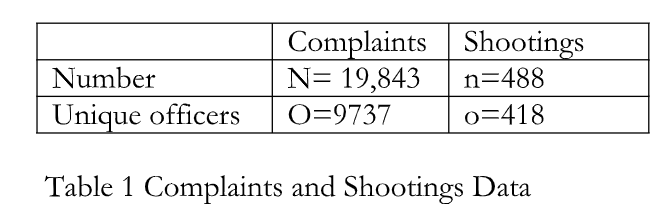
\includegraphics[width=0.4\textwidth]{figs/complaints_shootings_table_0.png}
\caption{table 1}
\end{figure}


In addition, the IPRA dataset reporting police-involved shootings has several
important limitations. Most notably, subsequent analysis by the City of
Chicago’s Office of Inspector General (OIG) found that IPRA did not follow best
practices in reporting use of force. Among other difficulties, IPRA relied on
CPD notifications, and did not independently verify that the Department had
provided all of the required weapons-discharge notifications.  At the same
time, the data appears relatively reliable. The OIG report compared the IPRA
reported shootings to those reported in CPD internal “tactical response
reports.” The comparison found that IPRA’s shooting data from September 2007 to
September 2014, which reported 488 “hit shootings,” had overreported by only
four shootings compared to the CPD tactical response reports, an error rate we
deemed to be within an acceptable range. 

We used IPRA incident-level shooting data to layer shooting events occurring
during the period under study onto the complaint network of co-listed officers
described above. For each shooting event, we recorded the date and location
(street address) of the shooting. We added this information to the complaint
network by adding the shooting event data to the officer-nodes in the network,
and in particular, to the officers who were recorded as having committed the
shootings. 

Fig. 2  Construction of the shooting network. On the left, the complaint network with shooting officers in red; on the right, the resulting shooting network.

In contrast to the complaint network, the shootings network is an event-focused
network. Some officers are involved with more than one shooting. A significant
fraction (86\%, n=358) of officers in the complaint network were associated
with only one shooting. A smaller fraction (12\%, n=51) of officer nodes were
associated with two shootings; 2\% (n=8) were involved in three shootings, and
one officer (Tracey Williams) was involved in five shootings. All of these
shootings are represented in the shootings network. 


\begin{figure}
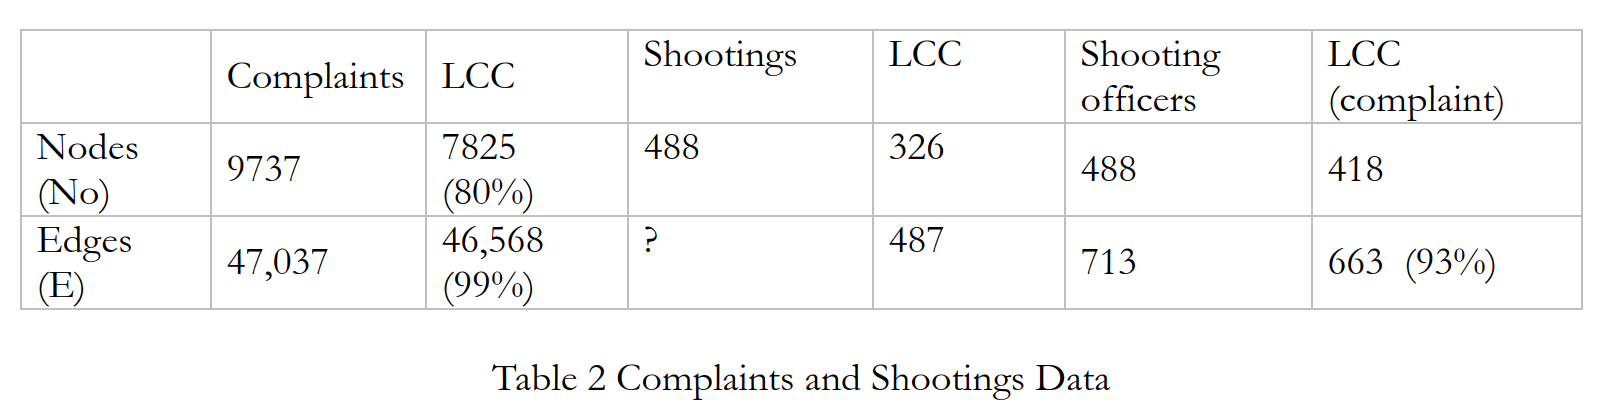
\includegraphics[width=0.4\textwidth]{figs/complaints_shootings_table.png}
\caption{table 2}
\end{figure}



%log_number,officer_name,unique_identifier,incident_date,incident_address,incident_year,specific_day_time


%Complaint_Number,Beat,Location_Code,Address,Street,Apartment,City_State_Zipcode,Incident_Datetime,Complaint_Date,Closed_Date,Full_Address,Investigator_Name,Investigator_Current_Assignment,Investigator_Rank,Investigator_Star,Investigator_Date_Appointed,Accused_Name,Accused_Birth_Yr,Accused_Gender,Accused_Race_Code,Accused_Date_Appointed,Accused_Current_Unit,Accused_Current_Rank,Accused_Star,Accused_Complaint_Category,Accused_Finding,Accused_Recommended_Discipline,Accused_Final_Finding,Accused_Discipline,PO_Witness_Name,PO_Witness_Gender,PO_Witness_Race,PO_Witness_Star,PO_Witness_Birth_Year,PO_Witness_Date_Appointed,Victim_Gender,Victim_Age,Victim_Race_Desc,Complainant_Gender,Complainant_Age,Complainant_Race_Desc

\subsection{Officer covariates}


% the roster data (as of April 2017):
%row_id,gender,race,birth_year,current_age,current_status,appointed_date,rank_no,current_rank,current_unit,unit_description,resignation_date,star1,star2,star3,star4,star5,star6,star7,star8,star9,star10,first_name,first_name_NS,last_name,last_name_NS,middle_initial,middle_initial2,suffix_name,merge,roster_1936-2017_2017-04_ID,UID,old_UID,link_UID

\begin{figure}
\centering
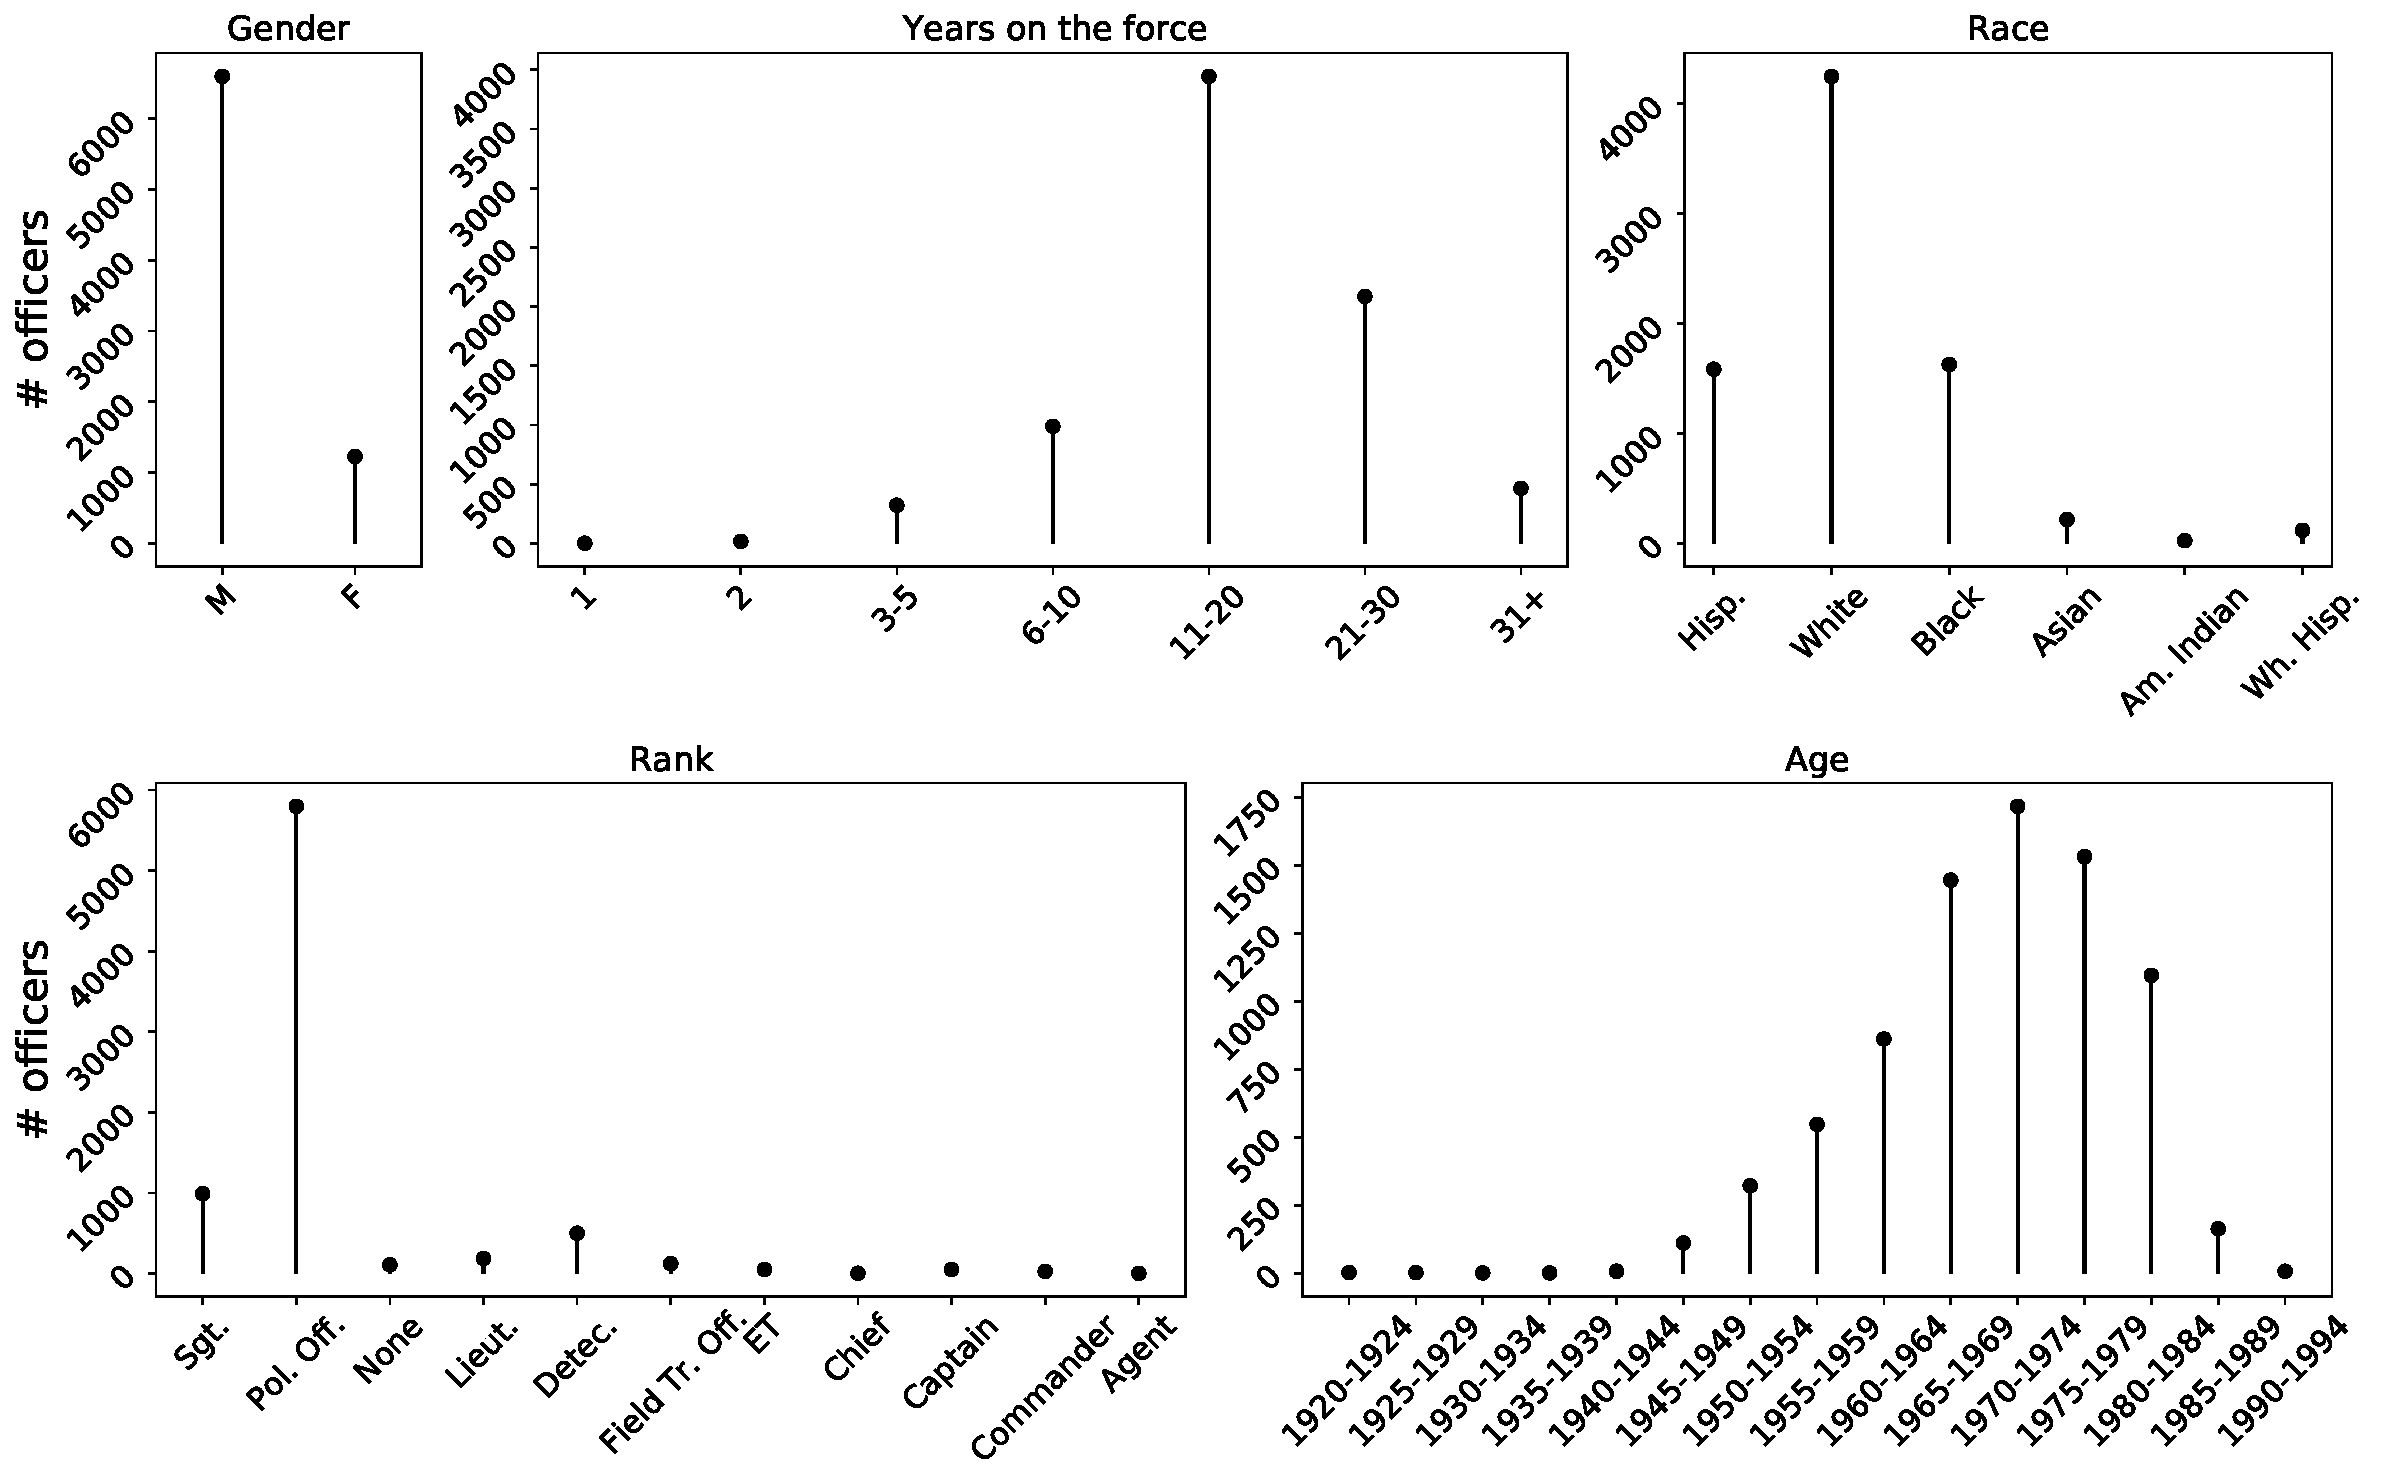
\includegraphics[width=\textwidth]{figs/data_inspection.pdf}
\caption{histograms of officer covariate}\label{fig:histograms}
\end{figure}

\begin{figure}
\centering
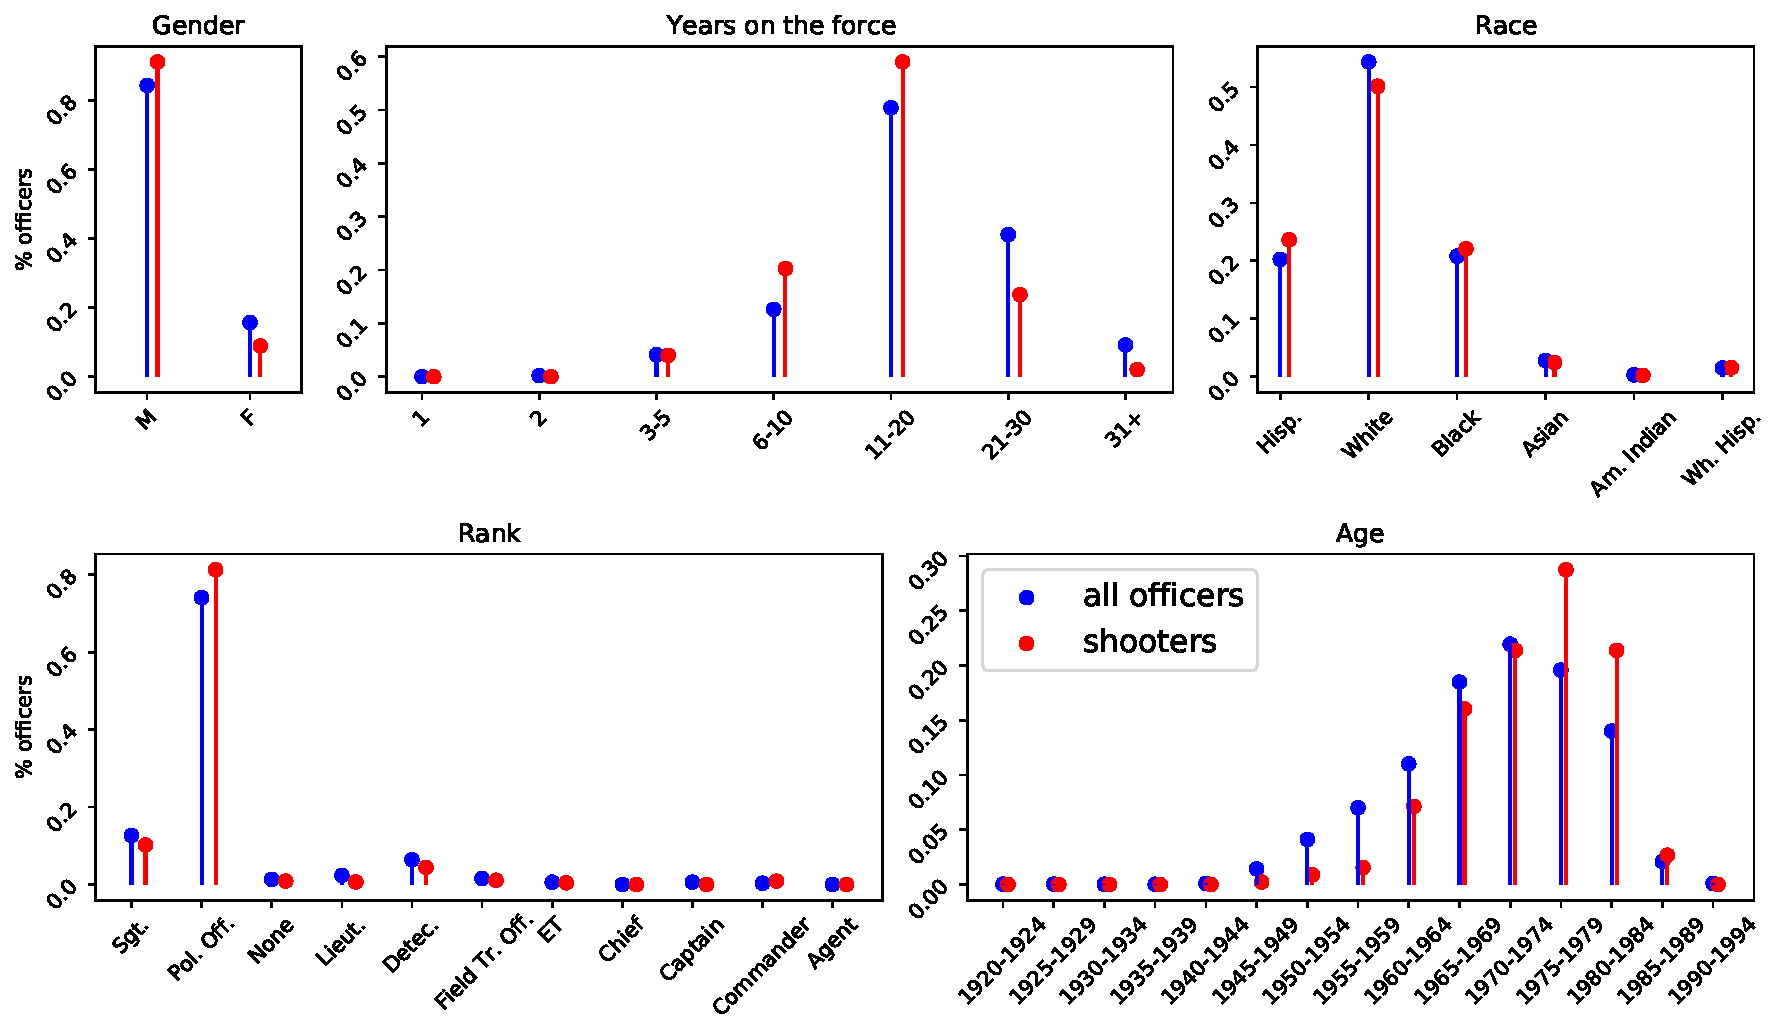
\includegraphics[width=\textwidth]{figs/shooters_relative.pdf}
\caption{histograms of shooter covariate (relative)}\label{fig:shooterhist}
\end{figure}

For each officer, the following information was available in our data: full
name, gender, race, birth date, appointment date, resignation date, rank, badge
number(s), and full unit membership history (including unit number, beginning date, and end date for each membership record).  
We used five of these variables---gender, race, birth date, rank, and number of years on the force since appointment---directly
as covariates in our statistical analyses. 
Figure \ref{fig:histograms} shows the distribution of values for each of these three covariates in the largest
connected component of the officer network. 
As we do not expect an officer's name or badge number to have any additional effect on their likelihood of shooting,
we did not use these variables as covariates. 
The sixth and final covariate for each officer that we considered is their unit membership history.
This section details how we processed each officer's unit membership
history to form a covariate for each officer, and then how we combined this with the previous covariates.

Our data contained a list of 242 unique units with a name and number. After removing
units that were not joined by any officer in the largest connected network component---many of them
old units that no longer exist---179 remained. We separated the units into groups
based on their function, to attempt to ensure a consistent effect on the likelihood of officer shootings in each group. 
The original unit reference data did not contain any actual description of unit function; for those
whose purpose was not clear from the name or whose name was missing entirely, 
we used the following sources to investigate unit function by number:
\begin{itemize}
\item Police directives from \url{http://directives.chicagopolice.org} and \url{https://directives.crimeisdown.com}
\item Investigatory Stop Report (ISR) counts by unit from the CPD annual reports 2017, 2018
\item Tactical Response Report (TRR) counts by unit from the CPD annual reports 2017, 2018
\item Chicago Data Portal crime counts: \url{https://data.cityofchicago.org/Public-Safety/Crimes-2001-to-Present/ijzp-q8t2}
\item Unit mentions in annual reports: \url{https://home.chicagopolice.org/statistics-data/statistical-reports/annual-reports/}
\item Specialized unit information: \url{https://home.chicagopolice.org/about/specialized-units/}
\item Organization charts: \url{https://www.chicago.gov/content/dam/city/depts/cpb/SuperintendentSearch/CPDOrgChart.pdf},
\url{https://home.chicagopolice.org/wp-content/uploads/2020/01/Department-Organization-for-Command-2019-July-19.pdf }
\end{itemize}

The resulting grouping of units is as follows. In total, we grouped the units into 
14 groups, plus an additional extra group for unit numbers appearing in the network whose
function and/or name are unknown. Some units appeared with duplicate numbers to others
(labelled ``dup.'' in the unit tables), but the duplicate name had the same meaning as the original
and did not influence grouping. 
\begin{description}
\item[Low Intensity / Unarmed Officers (49 units, 1 group, Table \ref{tab:desk})] Units
engaging in non-public-facing and
non-criminal-facing activities, units with unarmed officers,
and units performing low-intensity activities {\color{red}as judged by ISR / TRR}.
%
\item[District Units (27 units, 4 groups, Table \ref{tab:district})] Units that
correspond to patrols in the 25 districts\footnote{{\color{red} as of recent;
these change over time. How did we handle this?}} of Chicago. Of these, 25 are district-specific, and
the remaining two are city-wide. Given that Chicago is strongly racially and
economically segregated by district, we decided not to treat all district
patrols as a single unit type in the data, but rather clustered the district
units into 4 groups based on the number of homicides within each district
during the study period using the $k$-means algorithm \cite{xx}.  Figure
\ref{fig:districtclusters} shows the clustering of districts by number of
homicides, and Figure \ref{fig:districtelbow} shows the ``elbow plot'' used
to decide on the number of clusters. 
The two remaining units in this group are the bureau of patrol and
recruit training units; we treated officers in these units as city-wide
patrols, and used the average number of homicides city-wide to cluster these
units.
%
\item[Area Units (33 units, 3 groups, Table \ref{tab:area})] Units that operate within
the 6 areas\footnote{{\color{red} as of recent; these change over time. How did we handle this?}}  of
Chicago.  These include area patrols, youth divisions, gang and narcotics enforcement,
and violent and property crimes. We subdivided the area-based units similarly
to the district-based units due to the strong racial and economic segregation
of the city; in particular, we clustered the area units into 3 groups based on
the number of homicides in the area during the study period using the $k$-means
algorithm \cite{xx}. Figure \ref{fig:areaclusters} shows the clustering of
areas by number of homicides, and Figure \ref{fig:areaelbow} shows the ``elbow plot'' used
to decide on the number of clusters.
%
\item[Detail \& Controlled Zone Security (16 units, 2 groups, Table \ref{tab:controlzone}) ] Units whose officers
provide security of ``controlled zones'' (e.g., airports, courts, construction sites). Of these,
5/11 were labelled ``high/low-intensity'' {\color{red} based on ISR/TRR}.
%
\item[City-Wide Investigations (29 units, 2 groups, Table \ref{tab:citywide})] Units whose officers
perform city-wide detective, investigatory, and enforcement work. 
Of these, 16/13 were labelled ``high/low-intensity'' {\color{red} based on ISR/TRR}.
One unit worth mentioning is the Juvenile Intervention Support Center (JISC); although
we placed this unit in the ``low-intensity'' group, it 
could have equally been sorted into the ``high-intensity'' category, based
on its middling ISR and TRR counts.
%
\item[Special Operations (12 units, 2 groups, Table \ref{tab:specops})] Units whose officers
engage in special operations (e.g., SWAT, mounted, mobile strike force).
Of these, 9/3 were labelled ``high/low-intensity'' {\color{red} based on ISR/TRR}.
%
\item[Unknown (13 units, 1 group, Table \ref{tab:unk})] Units that are labelled as unknown in our dataset, and/or for which
we could not find any credible source of information detailing either the name or purpose of the unit. Given
naming/numbering patterns that are present in the remainder of the data, we hypothesize that units 271--5 are 
area-specific special operations units; but we could not verify this with any existing records. Although unit 45 had
a known label (``district reinstatement''), we could not find any source that described its purpose.

\end{description}



Next, we calculated the fraction of each officer's career spent being a member of
each of these groups. Note that officers can be a member of one or multiple units at the same time, so
these fractions do not necessarily sum to 1. The final ``unit membership'' covariate for each officer
was the vector of these 14 values (all between 0 and 1), one for each unit group.

Finally, we discretized the 6 covariates (gender, race, birth date, rank, number of years on the force since appointment,
and 14 fractions of time spent in each unit group) into bins:
\begin{description}
\item[Gender] 2 values were present in the data: male and female.
\item[Race] 6 values were present in the data: hispanic, white, black, asian/pacific islander, indian, and other. {\color{red} these correct?} 
\item[Birth Date] We grouped birth years together by 5 year intervals, resulting in {\color{red} XX bins}.
\item[Rank] {\color{red}XX values were present in the data: ...}
\item[Years on the Force] We grouped years on the force into 8 bins: 1, 2, 3-5, 6-10, 11-20, 21-30, 31-40, and 40+.
\item[Unit Membership] We discretized all 14 fractions into spacings of 0, 0.1, 0.2, etc. This created $10^{14}$ bins.
\end{description}
Combining all of these covariates, each officer was described by one of $xx$ unique values. Only officers with precisely
the same value were eligible to be swapped in the permutation test. 

Figure \ref{xx} shows the occupancy of bins

{\color{red} there were also units that appeared in our dataset but no officer was a recorded member of them in the network? LCC? here's the list of those}



\begin{figure}[h!]
\centering
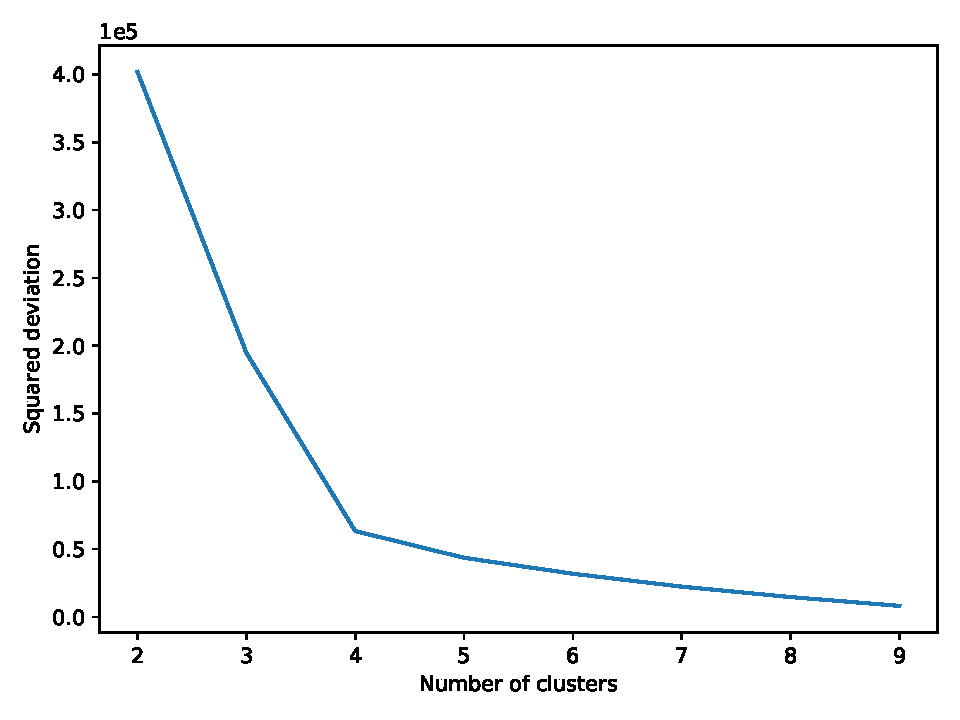
\includegraphics[width=0.75\textwidth]{figs/elbow-districts.pdf}
\caption{}\label{fig:districtelbow}
\end{figure}

\begin{figure}[h!]
\centering
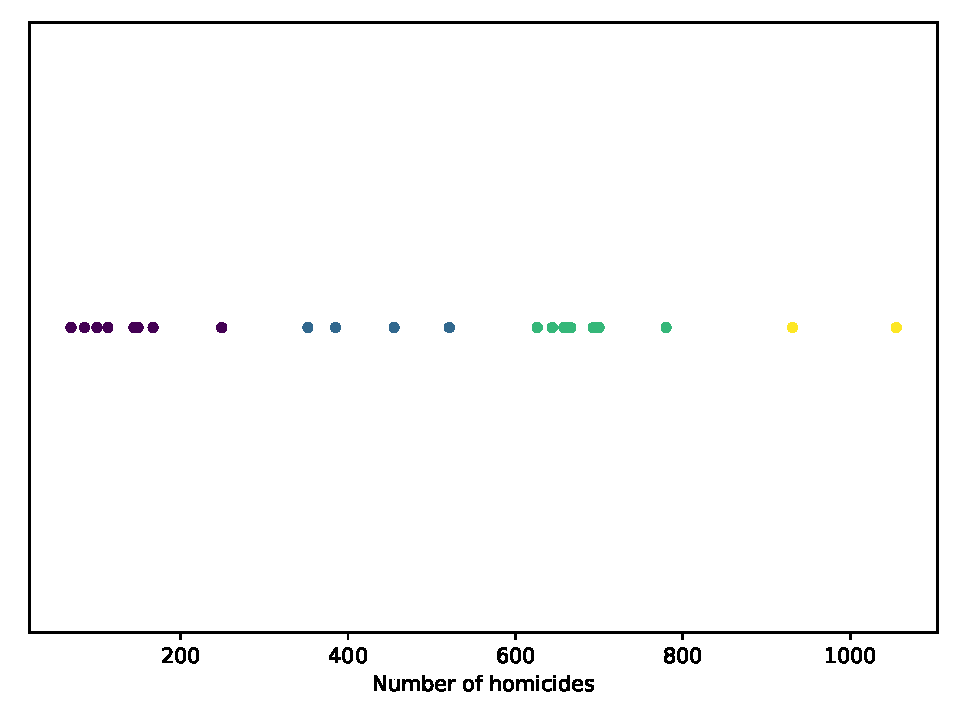
\includegraphics[width=0.75\textwidth]{figs/clusters-districts.pdf}
\caption{}\label{fig:districtclusters}
\end{figure}

\begin{figure}[h!]
\centering
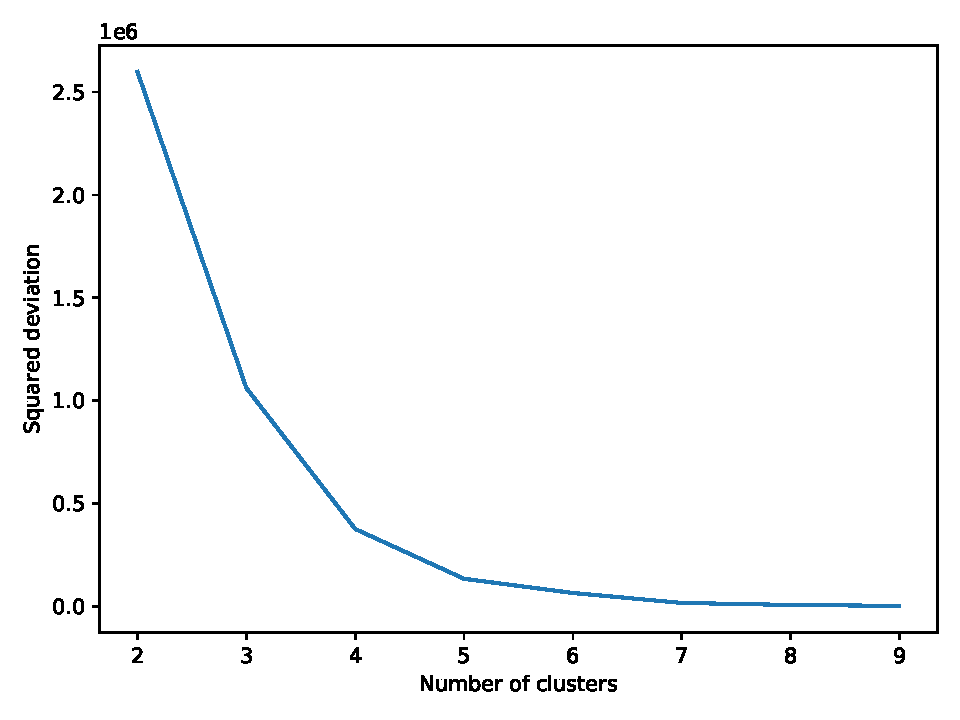
\includegraphics[width=0.75\textwidth]{figs/elbow-areas.pdf}
\caption{}\label{fig:areaelbow}
\end{figure}

\begin{figure}[h!]
\centering
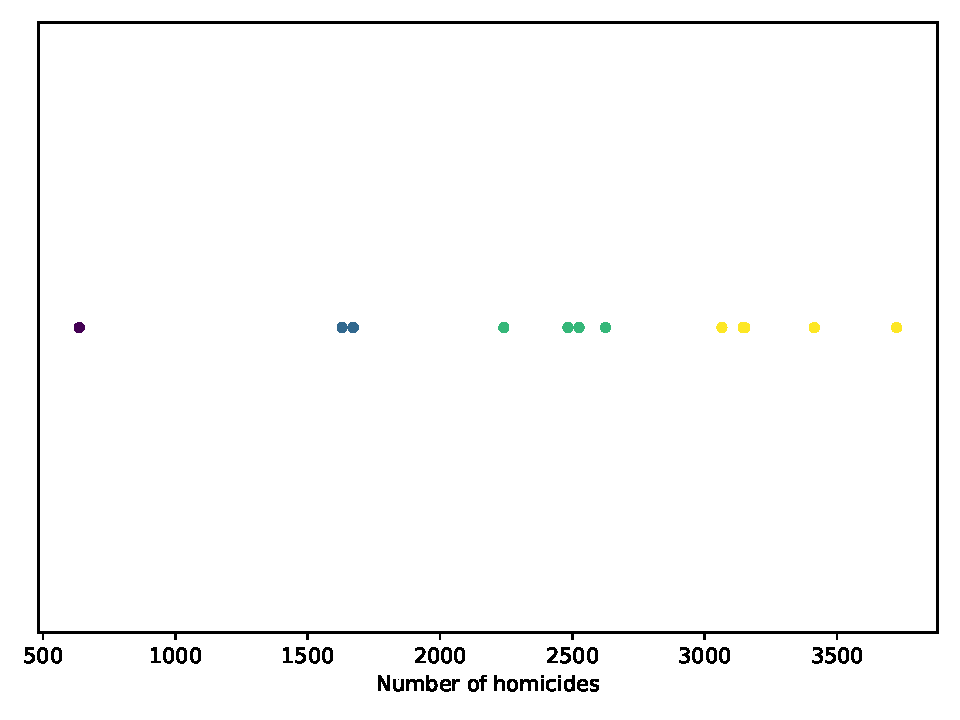
\includegraphics[width=0.75\textwidth]{figs/clusters-areas.pdf}
\caption{}\label{fig:areaclusters}
\end{figure}




\begin{table}
\tiny
\centering
\caption{}\label{tab:desk}
\begin{tabular}{|ll|}
\hline
Type: &	\textbf{Very Low Intensity \& Unarmed Officers} \\
\hline
Unit \# &	Unit Name \\
\hline
26	&Executive Officers Unit\\
86	&OEC-Police Dispatch\\
102	&Office Of News Affairs\\
111	&Office Of The Superintendent\\
112	&Bureau Of Professional Standards\\
114	&Legal Affairs Section\\
115	&CAPS Project Office\\
115	&Crime Control Strategies Section\\
116	&Deployment Operations Center\\
119	&Office Of International Relations\\
120	&Bureau Of Support Services\\
121	&Bureau Of Internal Affairs\\
123	&Human Resources Division\\
125	&Information Services Division\\
127	&Research And Development Division\\
128	&Professional Counseling Division\\
129	&Management And Labor Affairs Section\\
130	&Bureau Of Organizational Development\\
130	&Technology And Records Group\\
130	&Bureau Of Staff Services\\
163	&Records Inquiry Section\\
167	&Evidence And Recovered Property Section\\
169	&Police Documents Section\\
170	&CT \& ID Administration\\
172	&Equipment And Supply Section\\
175	&Telecommunications Unit\\
176	&Communication Operations Unit\\
214	&Freedom Of Information Section\\
216	&Deputy Chief Central Control Group\\
179	&Reproduction And Graphic Arts Section\\
231	&Medical Section\\
159	&Gun Registration\\
157	&Pub Housing Div Adm\\
601	&Det Div Admin.\\
944	&Cops Grant Recr Trng\\
165	&Field Inquiry Section\\
161	&General Support Division\\
139	&Asst Superintendent-Law Enforcement Operations (dup. CAPS)\\
140	&Office Of The First Deputy Superintendent\\
376	&Alternate Response Section\\
136	&Special Events Unit\\
166	&Field Services Section\\
126	&Inspection Division\\
147	&Senior Citizen Services\\
154	&Traffic Safety And Training\\
168	&Auto Pound Section\\
441	&Special Activities Section\\
135	&Chicago Alternative Policing Strategy (CAPS) Division\\
136	&CAPS\\
\hline
\end{tabular}
\end{table}



\begin{table}
\tiny
\centering
\caption{}\label{tab:district}
\begin{tabular}{|llll|}
\hline
Type: &	\textbf{District-Specific Units}  & &\\
\hline
Unit \# &Unit Name & Homicides & Cluster  \\
\hline
1	&District 001	&100	&0\\
2	&District 002	&455	&1\\
3	&District 003	&662	&2\\
4	&District 004	&693	&2\\
5	&District 005	&658	&2\\
6	&District 006	&780	&2\\
7	&District 007	&931	&3\\
8	&District 008	&644	&2\\
9	&District 009	&666	&2\\
10	&District 010	&700	&2\\
11	&District 011	&1055	&3\\
12	&District 012	&385	&1\\
13	&District 013	&385	&1\\
14	&District 014	&249	&0\\
15	&District 015	&626	&2\\
16	&District 016	&85	&0\\
17	&District 017	&149	&0\\
18	&District 018	&113	&0\\
19	&District 019	&144	&0\\
20	&District 020	&69	&0\\
21	&District 021	&455	&1\\
22	&District 022	&352	&1\\
23	&District 023	&144	&0\\
24	&District 024	&167	&0\\
25	&District 025	&521	&1\\
142	&Bureau Of Patrol	&447.52	&1\\
44	&Recruit Training Section	&447.52	&1\\
\hline
\end{tabular}
\end{table}



\begin{table}
\tiny
\centering
\caption{}\label{tab:area}
\begin{tabular}{|llll|}
\hline
Type: &	\textbf{Area-Specific Units}  & &\\
\hline
Unit \# &Unit Name & Homicides & Cluster  \\
\hline
71	&Youth Division Area1	&1672	&0\\
72	&Youth Division Area2	&2483	&1\\
73	&Youth Division Area3	&2241	&1\\
74	&Youth Division Area4	&2525	&1\\
75	&Youth Division Area5	&1630	&0\\
76	&Youth Division Area6	&637	&0\\
211	&Bureau Of Patrol - Area Central&3725	&2\\
212	&Bureau Of Patrol - Area South	&3414	&2\\
213	&Bureau Of Patrol - Area North	&3065	&2\\
214	&Deputy Chief - Area 4 (dup. Free. Of Info. Divn)&2625	&1\\
62	&Area 2 Pat Narc Prog	&2483	&1\\
63	&Area 3 Pat Narc Prog	&2241	&1\\
65	&Area 5 Pat Narc Prog	&1630	&0\\
66	&Area 6 Pat Narc Prog	&637	&0\\
311	&Gang Enforcement - Area Central&3151	&2\\
312	&Gang Enforcement - Area South	&3145	&2\\
313	&Gang Enforcement - Area North	&637	&0\\
314	&Gang Section - Area 4	&2625	&1\\
315	&Gang Section - Area 5	&1630	&0\\
612	&Violent Crimes DDA 1	&3151	&2\\
610	&Detective Area - Central	&3725	&2\\
620	&Detective Area - South	&3414	&2\\
621	&Prop Crimes DDA 2	&3145	&2\\
622	&Violent Crimes DDA 2	&3145	&2\\
630	&Detective Area - North	&3065	&2\\
631	&Prop Crimes DDA 3	&637	&0\\
632	&Violent Crimes DDA 3	&637	&0\\
640	&Detective Section - Area 4	&2625	&1\\
641	&Prop Crimes DDA 4	&2625	&1\\
642	&Violent Crimes DDA 4	&2625	&1\\
650	&Detective Section - Area 5	&1630	&0\\
651	&Prop Crimes DDA 5	&1630	&0\\
652	&Violent Crime DDA 5	&1630	&0\\
\hline
\end{tabular}
\end{table}



\begin{table}
\tiny
\centering
\caption{}\label{tab:controlzone}
\begin{tabular}{|ll|}
\hline
Type:	&\textbf{Detail \& Controlled Zone Security - High Intensity}\\ 
\hline
Unit \#	&Unit Name \\
\hline
704	&Transit Security Unit\\	
701	&Public Transportation Section \\
50	&Airport Law Enforcement Section - North \\ 
51	&Airport Law Enforcement Section - South \\
171	&Central Detention Unit	\\ 
\hline
Type:	&\textbf{Detail \& Controlled Zone Security - Low Intensity}\\ 
\hline
Unit \#	&Unit Name \\
\hline
143	&Court Section (dup .District Law)\\
261	&Court Section\\
284	&Admin School Securit\\
541	&FOP Detail\\
542	&Detached Services - Goverment Security\\
543	&Detached Services - Miscellaneous Detail\\
276	&OEC - Detail Section\\
57	&Traffic Section Detail Unit (dup. Detail Unit)\\
151	&Traffic Enforcement\\
152	&Loop Traffic Unit\\
145	&Traffic Section\\
\hline
\end{tabular}
\end{table}


\begin{table}
\tiny
\centering
\caption{}\label{tab:citywide}
\begin{tabular}{|ll|}
\hline
Type:	&\textbf{City-wide Investigations - High Intensity}\\ 
\hline
Unit \#	&Unit Name \\
\hline
189	&Narcotics Division\\
91	&Narc Special Enforce\\
92	&Narc General Enforce\\
156	&Gang Crime Section\\
393	&Gang Enforcement Division\\
188	&Bureau Of Organized Crime\\
193	&Gang Investigation Division\\
192	&Vice \& Asset Forfeiture Division\\
196	&Asset Forfeiture Investigation Section \\
740	&G/C Unit West\\
760	&G/C Unit North\\
710	&G/C Unit South\\
765	&Public Housing North\\
715	&Public Housing South\\
132	&Preven \& Neigh Div\\
606	&Central Investigations Division\\
\hline
Type:	&\textbf{City-wide Investigations - Low Intensity}\\
\hline
Unit \#	&Unit Name \\
\hline
79	&Special Investigations Unit\\
180	&Bureau Of  Detectives\\
184	&Youth Investigation Division\\
608	&Major Accident Investigation Unit\\
602	&Central Auto Theft\\
603	&Arson Section\\
603	&Bomb And Arson Division\\
384	&Juvenile Intervention Support Center (JISC)\\
191	&Intelligence Section\\
277	&Forensic Services Evidence Technician Sectn\\
377	&Forensic Services Unit - ET North\\
477	&Forensic Services Unit - ET South\\
177	&Forensic Services Division\\
\hline
\end{tabular}
\end{table}


\begin{table}
\tiny
\centering
\caption{}\label{tab:specops}
\begin{tabular}{|ll|}
\hline
Type:	&\textbf{Special Operations - High Intensity}\\ 
\hline
Unit \#	&Unit Name \\
\hline
55	&Mounted Unit\\
58	&Spec Func Canine\\
341	&Canine Unit\\
353	&Special Weapons And Tactics (SWAT) Unit\\
153	&Mobile Strike Force (dup. Special Functions Support Unit)\\
141	&Special Functions Division\\
146	&Canine Unit\\
241	&Troubled Building Unit\\
253	&Targeted Response Unit\\
\hline
Type:	&\textbf{Special Operations - Low Intensity}\\
\hline
Unit \#	&Unit Name \\
\hline
59	&Marine Operations Unit\\
442	&Bomb Squad\\
124	&Education And Training Division\\
\hline
\end{tabular}
\end{table}


\begin{table}
\tiny
\centering
\caption{}\label{tab:unk}
\begin{tabular}{|ll|}
\hline
Type: &	\textbf{Unknown} \\
\hline
Unit \# &	Unit Name \\
\hline
45  & District Reinstatement \\
52  & Unknown\\
54  & Unknown\\
56  & Unknown\\
64  & Unknown\\
661 & Unknown\\
720 & Unknown\\
271 & Unknown (Special Funcs Area 1?)\\
272 & Unknown (Special Funcs Area 2?)\\
273 & Unknown (Special Funcs Area 3?)\\
274 & Unknown (Special Funcs Area 4?)\\
275 & Unknown (Special Funcs Area 5?)\\
911 & Unknown \\
\hline
\end{tabular}
\end{table}




{\color{red}
\paragraph{Questions:}
\begin{itemize}
\item for years on the force -- this is appointment date minus what?  \tbo{end of study period minus appointment date}
\item what did we do with officers in the LCC who did not match?
\item did we include the UNK bins? how? -- yes, the unk fraction is treated as another "component" in the vector covariate
\item how did we deal with changing areas over time? changing districts?
\item 4 clusters in area unit plot, but only 3 unit bins
\end{itemize}
}

\begin{figure}[h!]
\centering
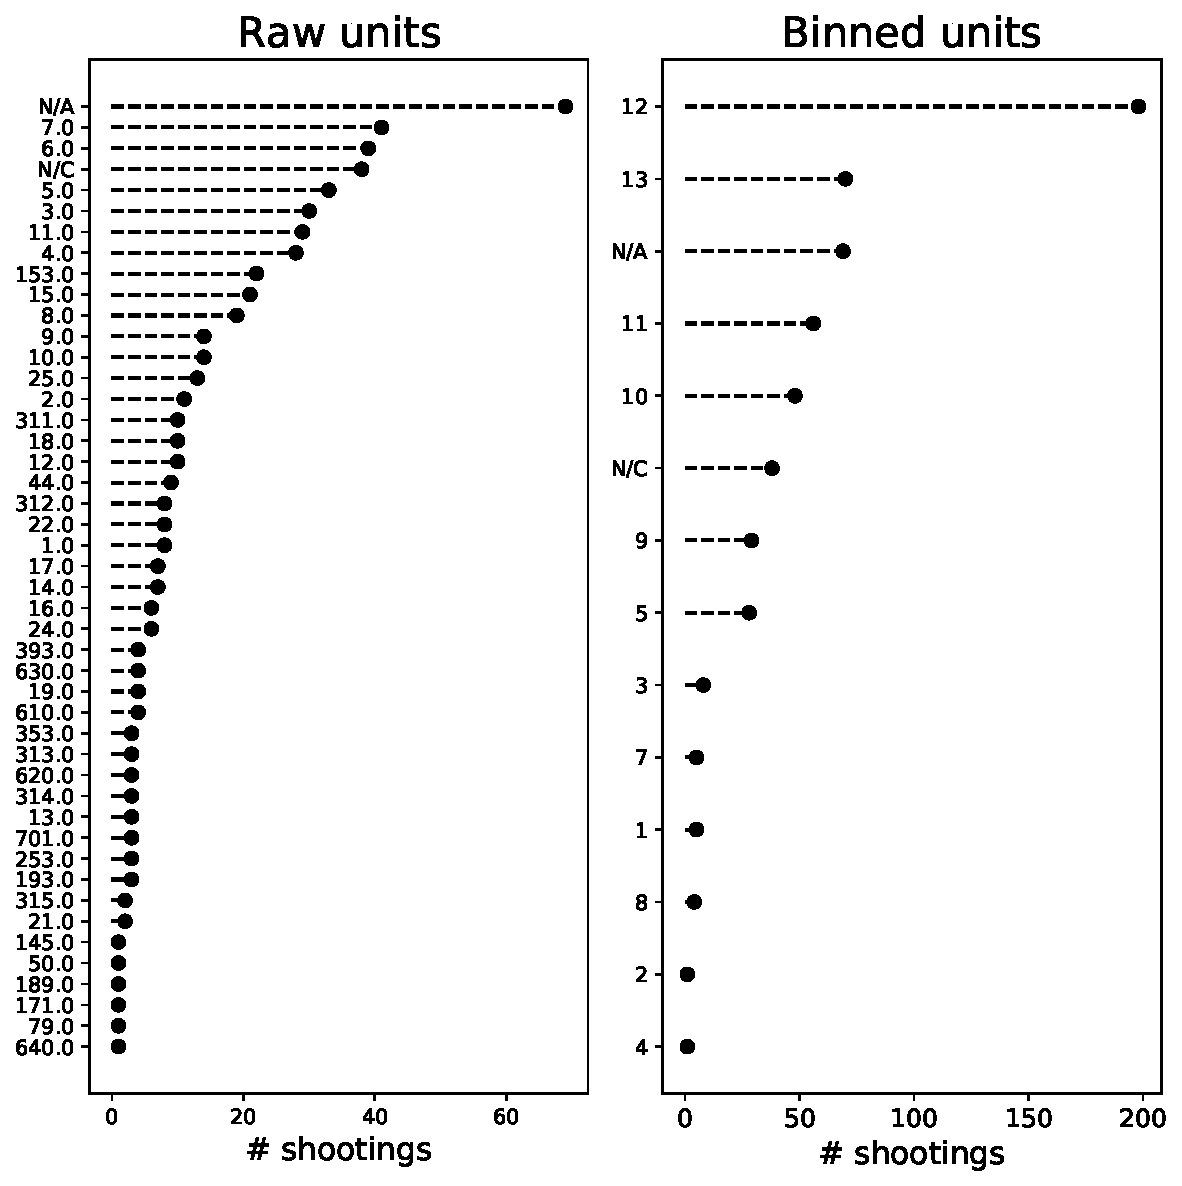
\includegraphics[width=0.75\textwidth]{figs/unit_plots.pdf}
\caption{}\label{fig:unitplots}
\end{figure}

Figure \ref{fig:unitplots} shows the number of shooting events
performed by officers in each unit and each unit bin during the study
period. To construct this figure, note that there are three
situations for each shooting event:
\begin{itemize}
\item The shooting officer is not present in the largest connected component of our network. 
These events are not included in the study, but we show them here labelled
``N/C'' (not counted). There are 38 such shooting events by 35/484 unique officers.
\item The shooting officer is present in the largest connected component but we could
not find a positive match for the officer in the roster (which has the unit history). 
These events are labelled ``N/A'' (not available). There are 69 such shooting events
by 57/484 unique officers.
\item The shooting officer is present in the largest connected component and there is
a positive match in the roster. There are 452 such shooting events by 392/484 unique officers.
Note that it is possible that a shooting officer is a member of multiple units simultaneously;
in this case, we add +1 to the shooting event counts for every unit the officer was a member of
at the time of shooting. But there is only one shooting event with such a situation, % Thomas Dineen 
where the officer was a member of both units 15 and 153.
\end{itemize}

